\documentclass[a4paper]{article}
\usepackage[resetfonts]{cmap}
\usepackage{lmodern}
\usepackage[slovak]{babel}
\usepackage[utf8]{inputenc}
\usepackage[T1]{fontenc}
\bibliographystyle{unsrt}
\usepackage{makeidx}
\usepackage{hyperref}
\usepackage{graphicx}
\usepackage{pdfpages}

\makeindex

\title{Karibská kríza}
\author{Tatiana Pohlodová}
\date{11. novembra 2023}

\begin{document}
% vlozenie zivotopisu
\shorthandoff{-}
\setcounter{page}{0}
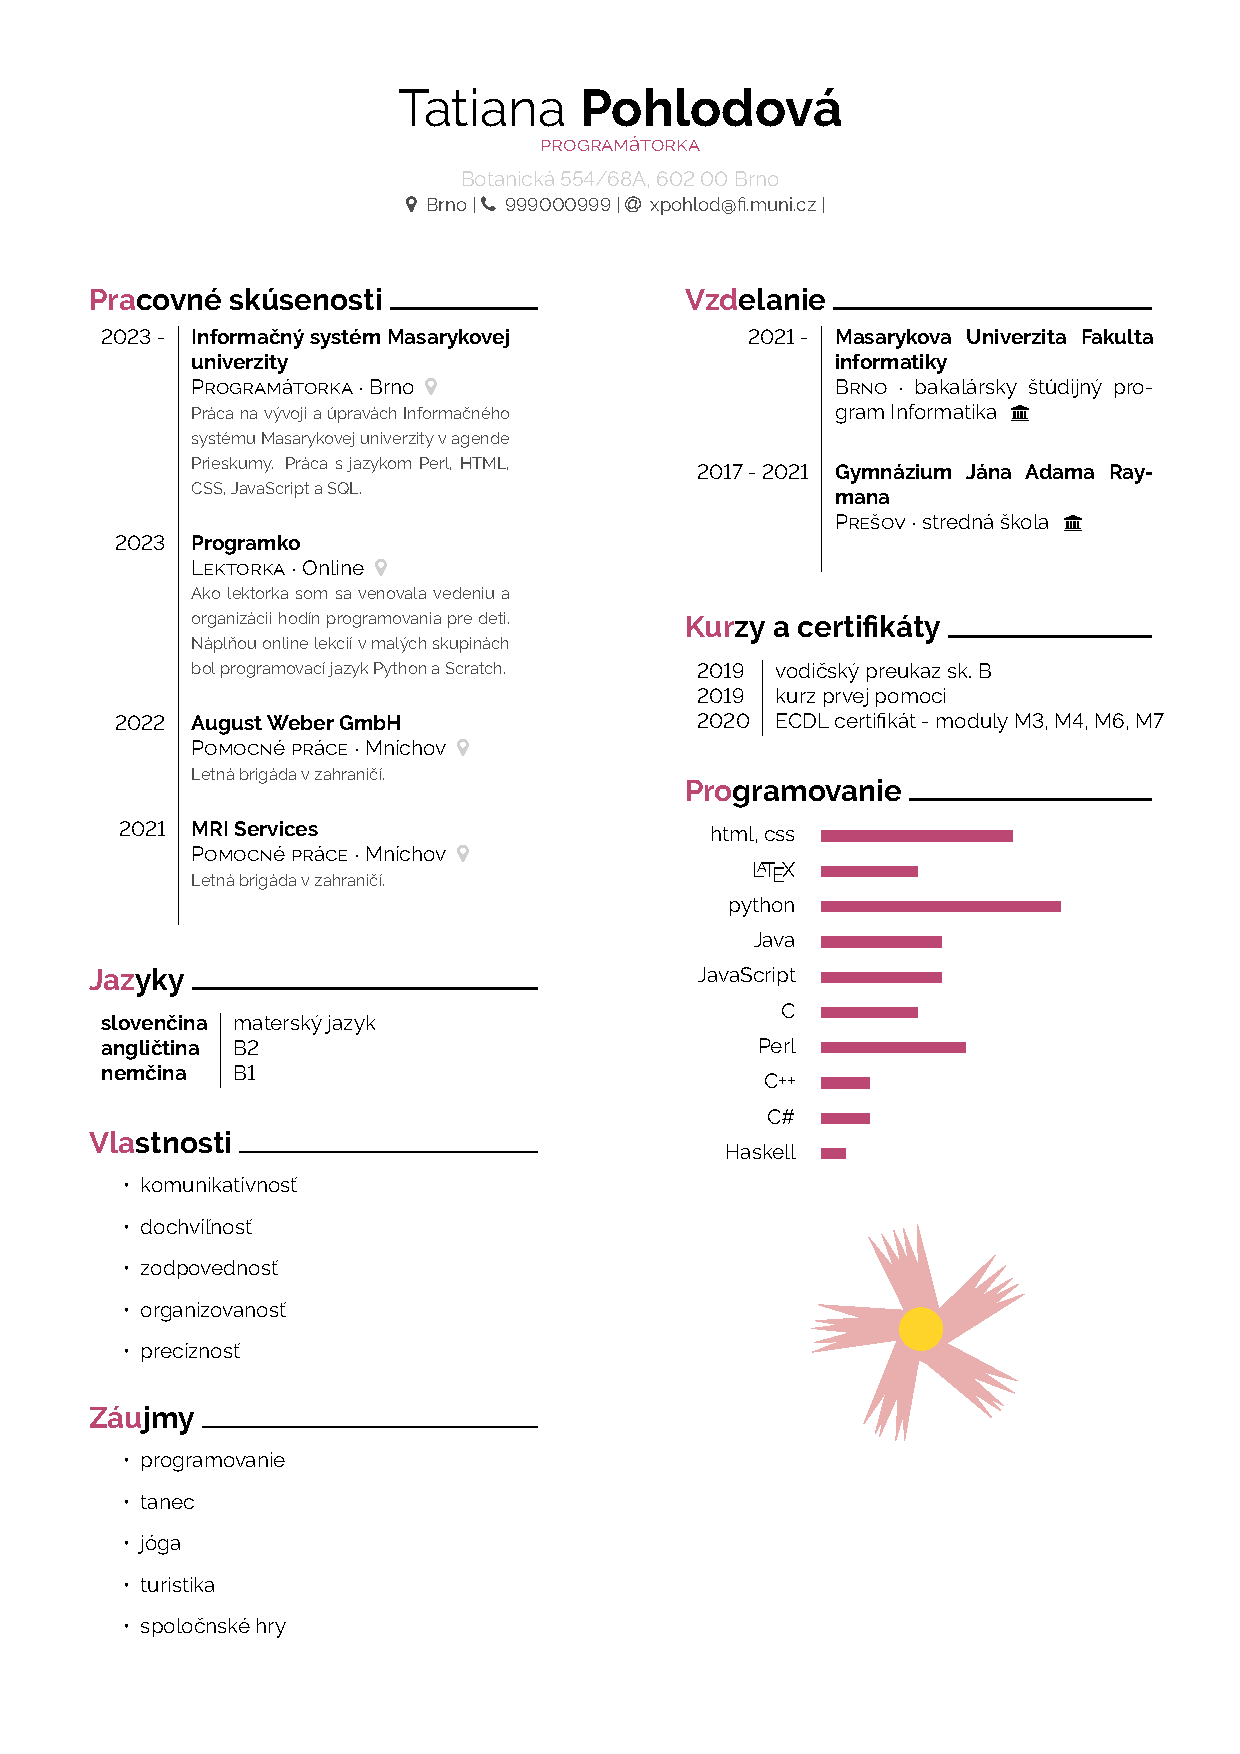
\includepdf[pages=-]{cv.pdf}

\maketitle

\section{Situácia~pred vypuknutím krízy}
Už od~formovania sfér vplyvu po~2. svetovej vojne boli vzťahy medzi ZSSR\index{ZSSR}~a USA\index{USA} komplikované. Krajiny medzi sebou súperili~v rôznych oblastiach, no najmä~o rozdelenie sfér vplyvu. V~roku 1947 stratili USA monopolné postavenie jedinej nukleárnej veľmoci~a začali preteky~o prevahu v zbrojení so ZSSR. Začalo sa obdobie vzájomného zastrašovania, pričom obe strany si uvedomovali, čo by mohol takýto otvorený jadrový konflikt\index{jadrový konflikt} znamenať.

\subsection{Situácia na Kube}
17.~februára~1959 bol menovaný za~predsedu novej reorganizovanej vlády Fidel Castro, ktorý zosadil Američanmi podporovaného Fulgencia Batistu. Od začiatku vo~vláde narastal vplyv komunistickej strany. \cite{mintomid} Castro dokonca ostro zasiahol proti pravicovým odporcom strany a~jeho vláda čoraz viac zasahovala do~súkromného sektoru hospodárstva. Opatrenia sa týkali najmä amerických firiem, ktoré na~Kube\index{Kuba} podnikali.

USA sa rozhodli pre~odvetu a~začali blokovať obchod s~Kubou. Tým odštartovali príklon Kuby k~Sovietskemu zväzu. Keď v~roku 1960 začala sovietska podpora Kuby, tak následne na to v~apríli toho roku ukončili svoju podporu USA. Potom začala masívna (najmä vojenská) podpora zo~strany ZSSR.

19.~októbra~1960, po~začatí znárodňovania\index{znárodňovanie} podnikov na~Kube, Američania odvolali svojho veľvyslanca a~úplne zablokovali obchod s~Kubou. Okrem toho začali prijímať voči Kube rôzne opatrenia a~začali organizovať tajné operácie. Vzťahy Kuby so~ZSSR sa kvôli týmto opatreniam čoraz viac prehlbovali a~posilňovali pozíciu Kuby ako predsunutej hliadky ZSSR na~západnej pologuli. \cite{mintomid}

3.~januára~1961 došlo k~úplnému prerušeniu diplomatických vzťahov s~USA, kvôli reakcii USA na~agrárnu reformu\index{agrárna reforma}. Opatrenia USA vyústili 16. apríla 1961 do~invázie v Zátoke svíň, pri~ktorej sa na~pobreží Kuby vylodili skupiny Američanmi vycvičených a~vyzbrojených kubánskych exulantov, ktorých cieľom bolo zosadenie Fidela Castra. \cite{13days} Fakt, že jediná obrana proti politike USA videla cez~ZSSR, priviedol Castra k~akceptovaniu komunizmu a~budovaniu štátu komunistického typu. Napriek všetkým nezhodám kubánski činitelia, hlavne Fidel Castro a~Ernesto „Che“ Guevara, neraz naznačili možnosť uvoľnenia väzieb so~ZSSR a~ochotu obnoviť vzťahy s~USA, avšak americká vláda na~tieto náznaky nereagovala.

\newpage

\section{Priebeh konfliktu}
\subsection{Rozmiestnenie sovietskych rakiet na~Kube}
Operácia Andyr, ktorej náplňou bolo vybudovanie sovietskych základní na~Kube, bola myslená ako odpoveď ZSSR na~rozmiestnenie amerických striel Jupiter v~Taliansku a~Turecku. Počas jari 1962 sa o~operácii definitívne rozhodlo a~na~Kubu bola vyslaná delegácia, ktorá mala vyjednať súhlas od~kubánskej vlády, ktorý nakoniec dostala. Operácia mala prebiehať tajne, aby mohol Chruščov\index{Chruščov} postaviť USA pred~hotovú vec a~aby mohli vyjednávať ako rovnocenní partneri. Jeho cieľom bolo najmä stiahnutie amerických striel Jupiter z~Turecka.

12.~júla~1962 sa začal presun vojenského materiálu na~Kubu. Celá operácia prebiehala tajne. Keď sa lode dostali mimo sovietskych vôd, boli tajne fotografované Američanmi. Američania z~týchto fotografií vedeli, že Sovieti prevážajú stíhačky, hliadkové člny a~nákladné autá, avšak nič nenaznačovalo prítomnosť jadrových zbraní\index{jadrové zbrane}. Rakety prevážali iba v~noci, aby celú operáciu udržali v~tajnosti. Vojaci boli oblečení ako civilisti. \cite{13days}

Na~sledovanie pohybu Sovietov na~území Kuby využívali Američania špionážne lietadlá U-2, ktoré lietali vo~vysokej nadmorskej výške a~boli vybavené kamerami s~vysokým rozlíšením. 28.~augusta zachytili kamery na~fotografie protilietadlové zbrane, čo znamenalo, že Sovieti chránia niečo dôležité. Nakoniec v~Národnom centre pre výskum fotografií objavili na~záberoch isté nezrovnalosti. Nakoniec zistili, že to boli balistické strely stredného doletu s~jadrovými hlavicami, ktoré mali dolet 3200 km a~mohli z Kuby zasiahnuť Washington, celé juhovýchodné územie USA a~ďalšie strategické ciele. 16.~októbra o~tomto zistení informovali prezidenta USA Johna Fitzgeralda Kennedyho a~skupinu okolo neho. Neskôr bola táto skupina nazývaná Výkonný výbor rady pre~národnú bezpečnosť.

\subsection{Odpoveď USA}
Kennedy\index{Kennedy} zvažoval, aké možnosti armáda má. Bol mu navrhnutý letecký útok na~zničenie rakiet, invázia na~Kubu alebo námorná blokáda. Nariadil zvýšenie počtu špionážnych letov. Zatiaľ nevedel o~plnej funkčnosti rakiet na~Kube ani o~plne vyzbrojených ponorkách, ktoré sa blížili k~pobrežiu.

Neskôr, keď mal k~dispozícii ďalšie zábery z~Kuby vedel, že odpoveď na~inváziu~na Kubu by bolo odpálenie rakiet, čo by znamenalo zničenie skoro celého územia USA. Avšak príprava naďalej pokračovala.

18. októbra sa prezident Kennedy stretol so~sovietskym ministrom zahraničných veci A. A. Gromykovom aby diskutovali o~povahe prevozu zbraní na~Kubu. Gromykov poprel prítomnosť akýchkoľvek útočných zbraní. Kennedy mohol dokázať opak, ale nekonfrontoval ho s~dôkazmi z~taktických dôvodov. Invázia na~Kubu bola zatiaľ odložená. Taktiež sa zrušil plán leteckého bombardovania, nakoľko zistili, že minimálne jedna sovietska balistická jednotka je pripravená. Nevedeli ani o~početných sovietskych vojenských jednotkách na~Kube.

\subsection{Stupňovanie napätia}
Spojené štáty sa nakoniec, cez~všetky dohady, rozhodli reagovať~na ohrozenie námornou blokádou\index{blokáda} Kuby. Bolo rozhodnuté, že to bude iba čisto vojenská blokáda a~Spojené štáty budú útočiť len v~prípade zlyhania tohto opatrenia. Hoci podľa medzinárodného práva je blokáda dôvodom na~začatie vojny, Kennedyho vláde to neprekážalo a~myslela si, že obyčajná blokáda nevyprovokuje Sovietsky zväz k~vojne. Prvé vojenské opatrenia sa začali 22.~októbra. Sovietske ponorky smerujúce na~Kubu začala blokovať americká protiponorková loď\index{loď!protilietadlová loď}.

Armáda USA bola v~najvyššej pohotovosti a~Kennedy mal prehovoriť k~americkej verejnosti v~ten istý deň. Informoval americký ľud o~prítomnosti sovietskych jadrových zbraní neďaleko pobrežia USA.

23.~októbra sa Moskva proti blokáde USA postavila a~označila ju za~ohrozenie svetového mieru a~zasahovanie do~cudzích záležitostí.

26.~októbra Chruščov prvý raz uznal existenciu rakiet na~Kube a~takisto prvý raz naznačil možnosť kompromisu. O~deň neskôr vzniesol ako základnú požiadavku stiahnutie amerických rakiet~z Turecka a Talianska. 

Ten istý deň, teda 27.~októbra, bolo nad~Kubou zostrelené americké prieskumné lietadlo s~majorom Rudolfom Andersonom, ktorý zahynul a~stal sa tak nakoniec jedinou obeťou konfliktu. To malo za~následok ďalší rozhorčený list adresovaný Nikitovi Chruščovovi, v~ktorom sa Kennedy rozčuľoval nad~zostrelením lietadla a~pokračujúcou výstavbou sovietskych základní na~Kube. V~liste Kennedy definitívne vyhlásil, že jeho snaha o~mierové riešenie končí a~dal Sovietskemu zväzu jasné ultimátum\index{ultimátum}, v~ktorom žiadal stiahnutie sovietskych rakiet do~48 hodín. Zároveň uviedol, že ak sa tak stane, Spojené štáty upustia od~blokády Kuby a~budú garantovať jej bezpečnosť.

\begin{figure}[htbp]
    \begin{center}
        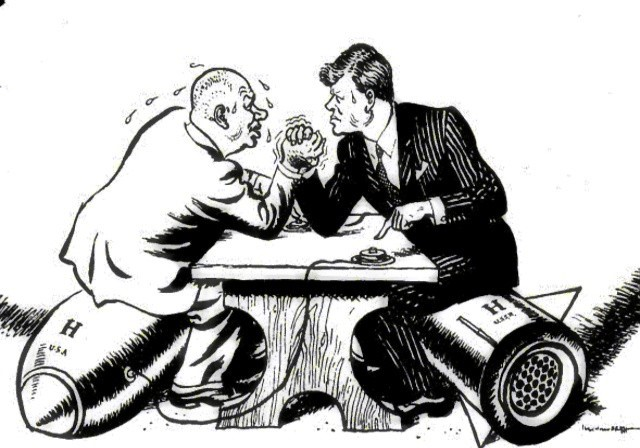
\includegraphics[width=0.55\textwidth]{karikatura}
    \end{center}
    \caption{Dobová karikatúra zobrazujúca Kennedyho a Chruščova. \cite{hn}} 
    \label{karikatura}
\end{figure}

\subsection{Vyriešenie krízy}
Kennedy Chruščovovi navrhol, že ak Sovieti urýchlenie odstránia a~odvezú z~Kuby rakety, tak USA ukončia blokádu Kuby a~nezrealizujú inváziu na~ostrov. Taktiež dodal, že USA po~čase stiahnu rakety Jupiter z Turecka, ale len za~podmienky, že ZSSR o tomto kroku pomlčí. Dal mu na~rozhodnutie 24 hodín. Medzitým sa napätie stupňovalo a~obe strany boli pripravené na~vypuknutie vojny. 28.~októbra, 2 hodiny pred vypršaním ultimáta Chruščov pristúpil~na 
podmienky. Do~konca roka 1962 bolo 60 balistických striel a 134 jadrových hlavíc odstránených z~Kuby. Napätie stále pretrvávalo, ale kríza bola ukončená.

\section{Dôsledky}
Dôsledkom tejto krízy bolo zriadenie tzv. horúcej linky\index{horúca linka} medzi Kremľom a~Bielym domom, ktorá mala zabrániť tomu, aby sa podobný scenár opakoval. \cite{dennikn} Taktiež výrazným spôsobom prispela k~začiatku rokovaní o~obmedzení jadrových zbraní. Prvá zmluva týkajúca sa zákazu jadrových pokusov bola podpísaná v~Moskve už v~roku 1963. Táto kríza taktiež prispela k~zmierneniu napätia vo~vzťahoch medzi a~ZSSR a~položila základy ďalšieho obdobia studenej vojny. Prehra Chruščova v~karibskej kríze výrazne oslabila jeho pozíciu v~ZSSR a~2~roky~po kríze ho skupina okolo Leonida Brežneva odstavila od~moci. \cite{hn}

\bibliography{literatura}

\begingroup
\let\clearpage\relax
\section*{\indexname}
\printindex
\endgroup

\end{document}